\subsection{Karakteristike operacionog pojačavača zavise od frekvencije ulaznog signala}

{Kao što je prethodno spomenuto izraz za izlazni napon operacionog pojačavača u otvorenoj sprezi je }

\begin{equation}
    V_{out} = A_o \cdot V_{in} = A_o \cdot (V^+ - V^-),
\end{equation}

{gde se smatra da je vrednost za $A_o$ konstanta ili u slučaju operacionog pojačavača u zatvorenoj sprezi zavisna od otpornika $R_1$ i $R_2$. Ovo nije tačno u praksi već pojačanje zavisi od frekvencije ulaznog signala. Sada se pojačanje modeluje kao funkcija prenosa prvog reda, odnosno}

\begin{equation}
    A_o(j\omega) = G(j\omega) = \frac{V_{out}(j\omega)}{V^+(j\omega) - V^-(j\omega)} = \frac{A_o}{1 + j\frac{\omega}{\omega_g}}.
\end{equation}

{Neophodno je razgraničiti pojmove u izrazu, $A_o(j\omega)$ je funkcija prenosa operacionog pojačavača čiji moduo $|A_o(j\omega)|$ određuje pojačanje operacionog pojačavača na određenoj frekveniciji ulaznog signala i čiji argument $arg(A_o(j\omega))$ određuje fazni pomeraj ulaznog signala na određenoj frekvenciji. U funkciji prenosa figuriše i $A_o$ koji predstavlja statičko pojačanje operacionog pojačavača, a $\omega_g$ predstavlja graničnu frekvenciju operacionog pojačavača. Do vrednosti $\omega_g$ se pojačanje smatra konstantnim, nakon $\omega_g$ ono opada.}

{\textit{\textbf{{Primer 1.}}} Pretpostavimo da je $A_o = 1 \,M\frac{V}{V}$, a da je $\omega_g = 20\pi \frac{rad}{s}$. Onda je funkcija prenosa operacionog pojačavača .}

\begin{equation}
    A_o(j\omega) = \frac{10^6}{1 + j\frac{\omega}{20\pi}}
\end{equation}

\begin{figure}[ht]
    \centering

    \begin{minipage}{0.48\textwidth}
        \centering
        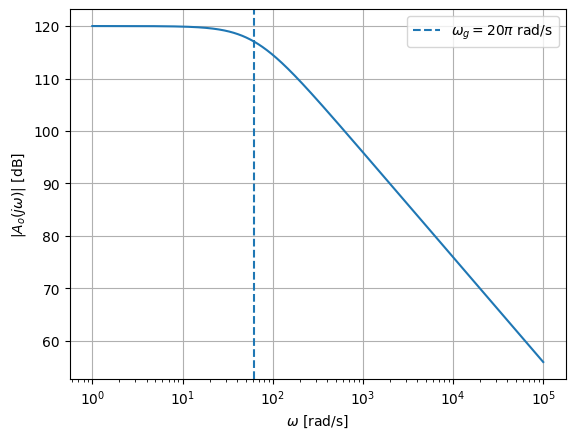
\includegraphics[width=\textwidth]{bode.png}
        \caption{Bodeov diagram}
        \label{fig:amplitudska}
    \end{minipage}
    \hfill
    \begin{minipage}{0.48\textwidth}
        \centering
        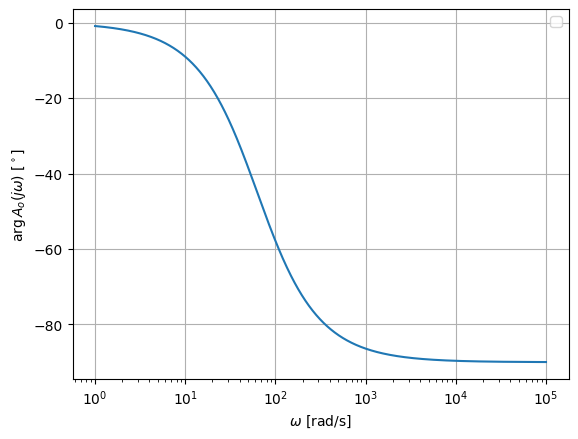
\includegraphics[width=\textwidth]{phase.png}
        \caption{Fazna karakteristika}
        \label{fig:fazna}
    \end{minipage}

\end{figure}

{Na graničnoj učestanosti $\omega_g$ dolazi do slabljenja signala u iznosu od 3 dB, što znači da posle te granice operacioni pojačavač više ne ostvaruje željeni izlaz.}

{Na osnovu bodeovog diagrama može se zaključiti da se operacioni pojačavač u ovakvoj izvedbi ponaša kao niskopropusni filtar i da povećanjem frekvencije ulaznog signala njegovo pojačanje tog signala na izlazu opada.}

{Uvodi se i parametar GBP operacionog pojačavača}

\begin{equation}
    GBP = A_o \cdot \frac{\omega_g}{2\pi} = A_o \cdot f_g \approx const.
\end{equation}

{Opisuje ponašanje pojačanja operacionog pojačavača pri promeni frekvencije ulaznog signala, odnosno za veće frekvencije pojačanje se smanjuje, ali GBP ostaje konstantan.}

{Kako je do sada obrađivan operacioni pojačavač u otvorenoj sprezi, neophodno je prokomentarisati šta se dešava sa frekvencijskim karakteristikama pojačavača kada se zatvori povratna sprega. Na slici \ref{fig:opamp_freq} je opet prikazano kolo invertujućeg operaciongo pojačavača na osnovu kojeg će biti izveden izraz za njegov izlaz.}

\begin{figure}[ht]
    \centering
    \begin{circuitikz}[american]
        \begin{scope}
            \ctikzset{tripoles/op amp/width=2.5,   % default 2.5
                    tripoles/op amp/height=2}    % default 2
            \node[op amp] (OA) at (0,0) {};
        \end{scope}
        \draw
            (OA.+) -- ++(-2,0) node[ground] {}
            (OA.-) to [R, l_=$R_1$] ++(-5, 0) to [V, l_=$V_{in}$] ++(0,-1.4) node[ground] {}
            (OA.out) -- ++(1,0) node[right]{$V_{out}$};

        \draw
            (OA.up) -- ++(0,1) node[above]{$+V_{cc}$};

        \draw
            (OA.down) -- ++(0,-1) node[below]{$-V_{cc}$};
        
        \coordinate (topV_minus) at ($(OA.-) + (-0.5, 2.5)$);
        \coordinate (startarrow) at ($(OA.-) + (-1.5, 0)$);

        \draw[->]
            (startarrow) -- ++(1,0) node[midway, above] {$I_1$};

        \draw[->]
            (topV_minus) -- ++(1,0) node[midway, above] {$I_2$};

        \node[circ] at ($(OA.-) + (-0.5,0)$) {};
        \node[below] at ($(OA.-) + (-0.5,0)$) {$V^-$};
        \node[circ] at ($(OA.+) + (-0.5,0)$) {};
        \node[below] at ($(OA.+) + (-0.5,0)$) {$V^+$};
        \node[circ] at (OA.out) {};

        \draw
            ($(OA.-) + (-0.5, 0)$) -- (topV_minus) to [R, l=$R_2$] ++(4,0) -- (OA.out);
        
    \end{circuitikz}
    \caption{Invertujući operacioni pojačavač}
    \label{fig:opamp_freq}
\end{figure}

\pagebreak

{Kako je funkcija prenosa operacionog pojačavača data sa izrazom $G(j\omega) = \frac{V_{out}(j\omega)}{V^+(j\omega) - V^-(j\omega)} = \frac{A_o}{1 + j\frac{\omega}{\omega_g}}$, neophodno je odrediti izraz za ulaz operacionog pojačavača, odnosno odrediti $V^+$ i $V^-$.}

{Kako je $V^+$ povezan na masu sledi}

\begin{equation}
    V^+ = 0.
\end{equation}

{Izraz za $V^-$ dobija se izjednačavanjem struja u kolu i sređivanjem izraza}

\begin{equation}
    \frac{V_{in} - V^-}{R_1} = \frac{V^- - V_{out}}{R_2}.
\end{equation}

\begin{equation}
    V^- = \frac{R_1V_{out} + R_2V_{in}}{R_1 + R_2}.
\end{equation}

{Gde je onda izraz za izlazni napon sledeći}

\begin{equation}
    V_{out} = -\frac{A_o}{1 + j\frac{\omega}{\omega_g}} \frac{R_1V_{out} + R_2V_{in}}{R_1 + R_2}.
\end{equation}

{Množenjem obe strane jednačine sa $(1 + j\frac{\omega}{\omega_g})(R_1 + R_2)$ i daljim sređivanjem dobija se odnos ulaza i izlaza invertujućeg operacionog pojačavača}

\begin{equation}
    \frac{V_{out}}{V_{in}} = \frac{-A_oR_2}{(R_1 + R_2)(1 + j\frac{\omega}{\omega_g}) + A_oR_1},
\end{equation}

\begin{equation}
    \frac{V_{out}}{V_{in}} = \frac{-A_oR_2}{R_1 + R_2 + A_oR_1 + j(R_1 + R_2)\frac{\omega}{\omega_g}}.
\end{equation}

{Izvlačenjem $R_1 + R_2 + A_oR_1$ iz imenioca dobija se sledeći izraz}

\begin{equation}
    \frac{V_{out}}{V_{in}} = \frac{\frac{-A_oR_2}{R_1 + R_2 + A_oR_1}}{1 + j(\frac{R_1 + R_2}{R_1 + R_2 + A_oR_1})\frac{\omega}{\omega_g}}.
\end{equation}

{Gde je sada moguće uvesti nove izraze za pojačanje i graničnu učestanost}

\begin{equation}
    \boxed{A_{inv} = \frac{-A_oR_2}{R_1 + R_2 + A_oR_1}}
    \quad i \quad
    \boxed{\omega_{inv} = \frac{R_1 + R_2 + A_oR_1}{R_1 + R_2} \omega_g}.
\end{equation}

{Finalni izraz za funkciju prenosa invertujućeg operacionog pojačavača je}

\begin{equation}
    \frac{V_{out}}{V_{in}} = \frac{A_{inv}}{1 + j\frac{\omega}{\omega_{inv}}}.
\end{equation}

{Izraz za neinvertujući operacioni pojačavač je sličan te neće biti izvođen već samo dat u finalnoj formi}

\begin{equation}
    \boxed{A_{noninv}
    =
    \frac{A_o(R_1 + R_2)}
    {R_1 + R_2 + A_oR_1}}
    \quad i \quad
    \boxed{\omega_{noninv}
    =
    \frac{R_1 + R_2 + A_oR_1}
    {R_1 + R_2}
    \omega_g}.
\end{equation}